\begin{enumerate}[label=\thesection.\arabic*.,ref=\thesection.\theenumi]
\numberwithin{equation}{enumi}

\item For an LTI system, the Bode plot for its gain defined as
\begin{align}
	G(s) = 20\log\abs{H(s)}
	\label{eq:ep18btech11016_gain}
\end{align}
is as illustrated in the Fig. \ref{fig:ep18btech11016_bode}. Find the corner frequencies $\omega_{01}$ and $\omega_{02}$ from the plot.
\begin{figure}[ht!]
\centering
    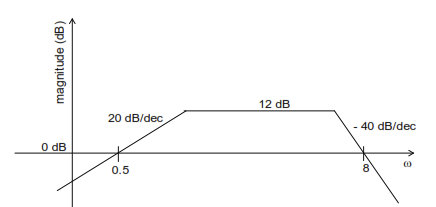
\includegraphics[width=\columnwidth]{./figs/ep18btech11016_fig1.png}
    \caption{}
    \label{fig:ep18btech11016_bode}
\end{figure}

\solution
The corner frequencies can be calculated as follows:
\begin{align*}
    slope = \cfrac{M_2 - M_1}{log\omega_2 - log\omega_1}\\
\end{align*}

Therefore for $\omega_{02}$,\\
-40 = \cfrac{0 - 12}{log8 - log\omega_{02}}\\
log8 - log$\omega$_{02} = \cfrac{12}{40}\\
log$\omega_{02}$ = log8 - \cfrac{12}{40}\\
$\omega_{02}$ = 4\\

And for $\omega_{01}$,\\
20 = \cfrac{0 - 12}{log0.5 - log$\omega_{01}$}\\
log0.5 - log$\omega_{01}$ = \cfrac{-12}{20}\\
log$\omega_{01}$ = log0.5 + \cfrac{12}{20}\\
$\omega_{01}$ = 2\\
So, the corner frequencies are $\omega_{01}$=2 and $\omega_{02}$ = 4.\\

\item Find the transfer function from the calculated frequencies.\\
\solution
By looking to the plot, we can say that since the initial slope is +20, there must be a zero at the origin.\\
At $\omega_{01}$, the change in slope is -20dB, so their exists one pole at this frequency.\\
At $\omega_{02}$, the change in slope is -40dB, so their exists two pole at this frequency.\\
The denominators have the form (1 + \cfrac{s}{\omega})

So, the denominator of the transfer function is\\ $(1 + \cfrac{s}{2})(1 + \cfrac{s}{4})^2$\\
Therefore, the transfer function is,
\begin{align*}
    \cfrac{cs}{(1 + \cfrac{s}{2})(1 + \cfrac{s}{4})^2} 
\end{align*}
here c is some constant\\

\item Compare the above calculated transfer function with one of the options that best represents it.
\begin{multline*}
    (A) \cfrac{2s}{(1+0.5s)(1+0.25s)^2}\hspace{0.5cm}
    (B) \cfrac{4(1+0.5s)}{s(1+0.25s)}
\end{multline*}
\begin{multline*}
    (C) \cfrac{2s}{(1+2s)(1+4s)}\hspace{0.5cm}
    (D) \cfrac{4s}{(1+2s)(1+4s)^2}
\end{multline*}
\solution
From the above given option, we can see that option (A) best represents our transfer function.
\begin{align*}
     \cfrac{2s}{(1+0.5s)(1+0.25s)^2}
\end{align*}{}

\item Verify the above plot by plotting the transfer function.\\
\solution
The bode plot is:
\begin{center}
    \begin{figure}[!h]
    \centering
    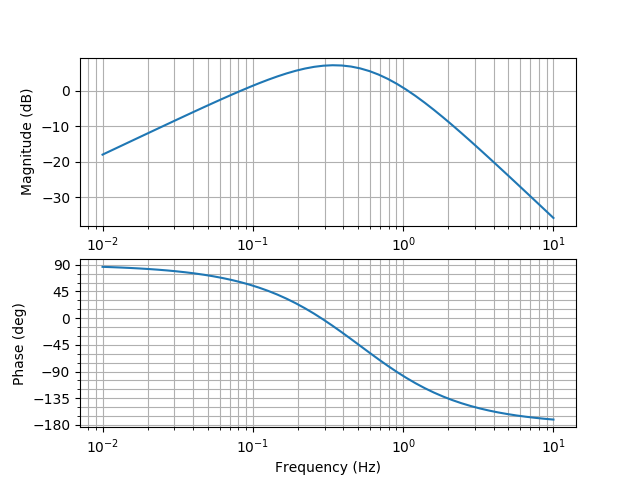
\includegraphics[width=\columnwidth]{./figs/ep18btech11016_fig2.png}
    \caption{Plot of G(s)}
    \label{fig:ep18btech11016_fig2}
    \end{figure}
\end{center}
The plot was plotted using the following code:
\lstinputlisting{./codes/ep18btech11016.py}

\end{enumerate}
